\chapter{Introduction}
\label{chap:intro}

\section{Background}


%TODO: Diagram of net. arch.
Computer networks have two classes of elements: the \textit{end hosts} that
generate packets and the \textit{routers}\footnote{We use the term router to
refer to both switches and routers in this disseration.} that forward these
packets between the end hosts. Historically, the Internet was architected so
that most of the complexity resided in the end hosts, while the routers
themselves were simple. According to Clark~\cite{design_philosophy}, this
architecture was a result of the overarching design goal of the Internet: the
ability to easily interconnect existing networks with disparate network
architectures (\eg long-haul networks, local-area networks, satellite networks,
and radio networks) while providing acceptable end-to-end connectivity. Quoting
Clark, "The Internet architecture achieves this flexibility by making a minimum
set of assumptions about the function which the net will provide."

The minimum functionality assumed of and provided by the network was
best-effort and unreliable packet forwarding. Notably absent from a router's
feature set were reliable packet delivery, packet prioritization, monitoring
features to attribute a router's resource usage to specific end hosts, and
security features to detect network breaches. As a result, the early routers
were singularly dedicated to packet forwarding. A minimal router feature set
made it simpler to design high-speed routers and helped broaden the Internet's
reach by interconnecting existing networks with minimum friction. But, it
sidelined other goals~\cite{design_philosophy} such as improving network
performance, security, and monitoring.
 
Today, four decades after ideas underlying the Internet were first
published~\cite{cerf74}, it is clear that routers need to do much more than
forward packets for at least two reasons. First, once the basic goal of
interconnecting different networks is achieved, other goals like performance,
security, and monitoring rise in prominence.  Second, many large-scale private
networks (\eg datacenters, private wide-area networks, enterprise networks) do
not need to concern themselves with interconnecting disparate networks as the
Internet had to and hence can expect more from their network. As a result, a
typical router today implements many features beyond packet forwarding,
pertaining to security (\eg access control), monitoring (\eg counting the
number of packets belonging to each flow transiting the router), and
performance (\eg priority queues).

However, despite the feature creep in routers, there's little consensus between
network operators and router vendors on a router's feature set. Inevitably,
there are network operators whose needs fall outside their router's feature
set. But because today's fastest routers are built out of specialized
forwarding hardware, they are largely {\em fixed-function} in that their
functionality cannot be changed once the router has been built. In such cases,
the operator has no alternative but to wait two--three years for the next
generation of the router hardware---best illustrated by the lag time between
the standardization and availability of new overlay protocols~\cite{vxlan,
nvgre}.

As a result, the rate of innovation in new router algorithms is outstripping
our ability to get these algorithms into production routers, especially those
routers that run at speeds in excess of a Tbit/s.
Figure~\ref{fig:router_algos} shows a timeline of prominent router algorithms
that have been developed since the 1980s. Of these, only a handful are
available in production routers because there is no way to program a new router
algorithm on a production router.
%TODO: What is a production router?

\begin{figure}
\centering
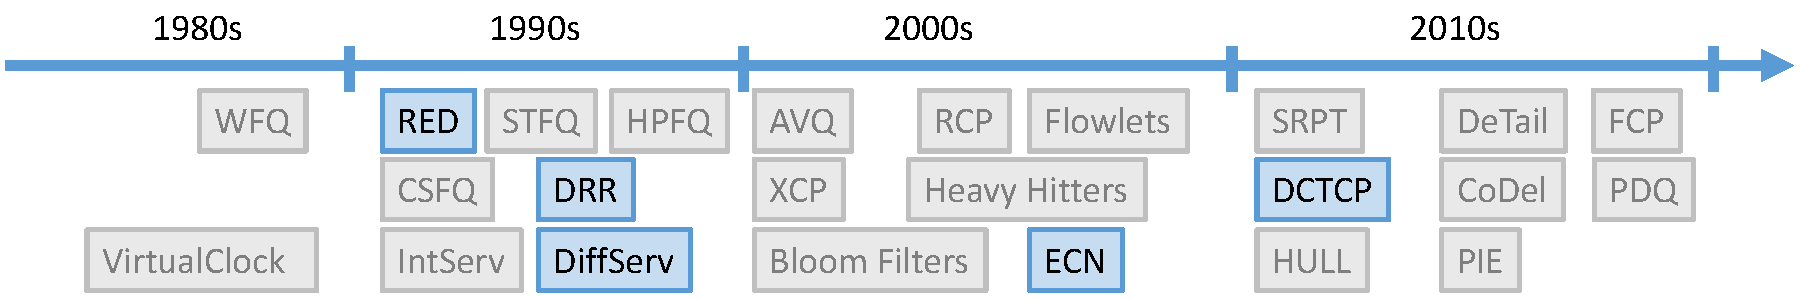
\includegraphics[width=\columnwidth]{router_alg_timeline.pdf}
\caption{Timeline of prominent router algorithms since the 1980s. Only the ones
shaded in blue are available on production routers today.}
\label{fig:router_algos}
\end{figure}

As an operator who wants to introduce new functionality in their network, what
are the operator's choices? One is to give up on changing routers altogether
and make all the required changes at end hosts as the original Internet did.
However, relying solely on end hosts results in solutions that are cumbersome
or suboptimal. As a first example, imagine measuring the queuing latency at a
particular hop in the network. One could do this by collecting end-to-end ping
measurements between a variety of vantage points and then fusing these
measurements together to estimate per-hop queueing latency. Not only is this
indirect, it is also inaccurate relatively to directly instrumenting the router
at that hop to measure its own queueing latency. As a second example, consider
the problem of congestion control, which divides up a network's capacity fairly
among competing users. There are many in-network solutions to congestion
control~\cite{xcp, rcp}, which outperform the end-host-only approaches to
congestion control used today~\cite{cubic, compound}. But, there is no way to
deploy them. 

Another alternative is to use a \textit{software router}: a catch-all term for
a router built on top of some \textit{programmable} substrate, such as a
general-purpose CPU~\cite{click, routebricks}; a network processor, a CPU with
an instruction set tailored to packet processing~\cite{ixp4xx, ixp2800}; a
GPU~\cite{packetshader}; or an FPGA~\cite{netfpga}.
Figure~\ref{fig:router_evolution} tracks the evolution of aggregate capacity of
software routers and compares them to the fastest routers known at a any point
in time. The figure shows two trends. First, up until the mid 90s, software
routers were in fact the fastest routers; the early routers~\cite{imp} were
minicomputers loaded with forwarding software. However, since the mid 90s,
growing demands for higher link speeds, fueled by the Internet's explosive
growth, have meant that the fastest routers are now built out of dedicated
hardware, specialized for packet forwarding. As a result of hardware
specialization, the performance of these routers is between 10 and 100 $\times$
better than software routers.  This performance improvement is because software
routers do not fully exploit the large degree of parallelism available in
packet processing: within the processing of a single packet, across packets at
different ports, and pipeline parallelism when carrying out different functions
on the same packet. However, hardware specialization comes at a cost: because
these routers are built out of specialized hardware, they are fixed-function
devices that can not be reconfigured in the field.

Recent work in software-defined networking~\cite{openflow} (SDN) and
programmable switching chips~\cite{rmt, xpliant, flexpipe} has endowed fast
routers with limited flexibility. SDN allows operators to program the network
control plane, which is the part of the network that computes a network's
routing tables, by moving route computations out of the routers and on to a
programmable server. Programmable switching chips allow operators to program
parts of the data plane, which is the part of the network that forwards packets
based on the routing tables, such as packet header manipulations that do not
modify router state.  However, these solutions are still not sufficient to
express the grayed-out algorithms shown in Figure~\ref{fig:router_algos}
because (1) these algorithms programmatically manipulate router state and (2)
they require flexibility in packet scheduling, which is untouched by both SDN
and programmable switching chips.

\begin{figure}
\centering
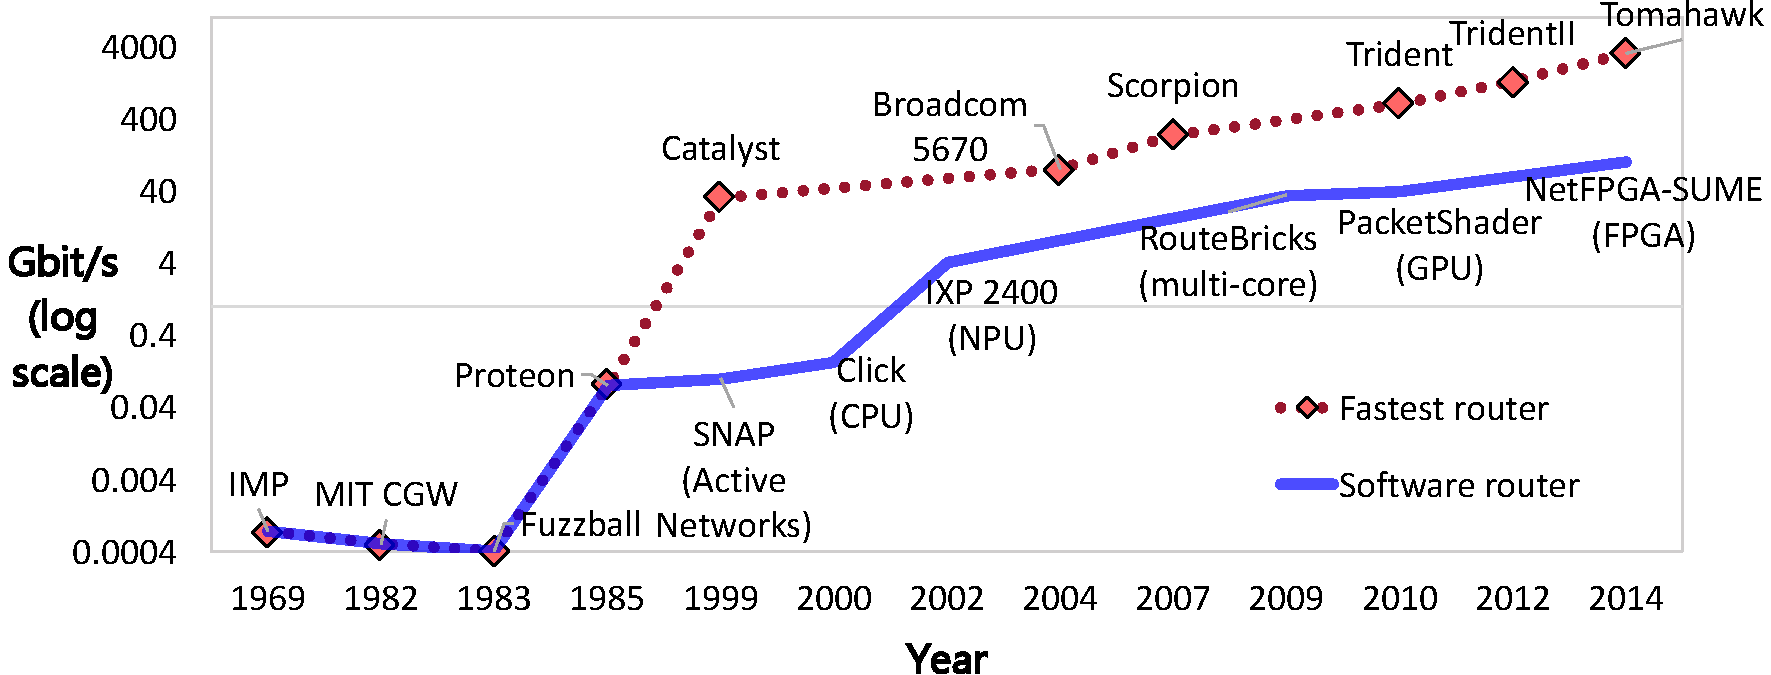
\includegraphics[width=\columnwidth]{router_evolution.pdf}
\caption{Aggregate capacity of routers since the first router on the ARPANET in
1969~\cite{imp}. Until the mid 90s, software routers were sufficient. Since
then, however, the fastest routers have been built out of dedicated hardware.}
\label{fig:router_evolution}
\end{figure}

\section{Primary contributions}

This dissertation considers the problem of building routers that approach the
speeds supported by today's fastest fixed-function routers, while also being
programmable. In particular, the thesis of this disseration is that it is
possible to design router hardware that is both fast and programmable, as long
as we restrict ourselves to specific classes of router functionality. It is
this specificity that allows us to resolve the programmability-performance
tension; indeed, our designs provide a much more restricted form of
programmability than a Turing-complete processor. The challenge here is to pick
classes of router functionality that are simultaneously (1) practically useful
to network operators, (2) broad enough to cover a range of current and future
use cases within that class, and yet (3) narrow enough to permit a high-speed
hardware implementation. We will describe high-speed programmable hardware
designs and their corresponding programming models in software for three
classes of router functionality: stateful data-plane algorithms, packet
scheduling, and scalable network measurement.

\subsection{Stateful data-plane algorithms}
Domino (Chapter~\ref{chap:domino}) is a system to program \textit{data-plane
algorithms} on high-speed router hardware. Data-plane algorithms operate on a
sequeunce of packets, doing a bounded amount of work per packet and
manipulating a bounded amount of router state in the process.  They include
algorithms for managing the router's buffer, load balancing, and in-network
congestion control.

High-speed data-plane programming poses two challenges: (1) what hardware
instructions are required to support programmable state modification at the
router's line rate and (2) what is the right programming model? In addressing
each challenge, Domino makes two new contributions:
\begin{CompactEnumerate}
\item \textit{Atoms} capture a router's instruction set. They specify atomic
units of packet processing provided by the router hardware, \eg an atomic
counter or an atomic test-and-set. Atoms are atomic in that all state updated
by an atom is visible to the next packet arriving at that atom.
\item \textit{Packet Transactions} provide a programming model. A packet
transaction is an atomic and isolated block of code capturing an algorithm's
logic. It provides the semantics that any visible state is equivalent to a
serial execution of packet transactions in the order of packet arrival---akin
to an infinitely fast single-threaded router. Packet transactions are
expressive and capture many important data-plane algorithms. Further, their
serial semantics shield programmers from the hardware's parallelism, instead
enlisting the Domino compiler to transform a serial packet transaction to a
parallel atom pipeline.
\end{CompactEnumerate}

For the first time, atoms and packet transactions allow us to program several
algorithms from Figure~\ref{fig:router_algos} (\eg the Adaptive Virtual
Queue~\cite{avq} active queue management algorithm, the CONGA~\cite{conga} load
balancing algorithm, bloom filters for measurement, and count-min sketches for
detecting heavy hitters~\cite{opensketch}) on speeds approaching high-speed
routers. P4~\cite{p4}, a packet-processing language that is emerging as an
industry standard for programming router chips now supports the packet
transaction abstraction.  P4 programmers can now use an @atomic annotation
around a block of statements to specify that the block must execute atomically.

%% Talk about the new atoms that the Domino created as the lasting contribution from the work

\subsection{Packet scheduling}

Packet scheduling is an important determinant of network performance. The
choice of scheduling algorithm is tied to a network's overarching goals. For
instance, an algorithm that divides link capacity fairly is ideal in a
multi-tenant setting~\cite{wfq}, while the shortest remaining processing time
algorithm is ideal for a single tenant who desires low flow completion
time~\cite{pFabric}. Today's routers provide a fixed set of scheduling
algorithms and do not allow an operator to program scheduling to suit their
needs.

Routers lack programmable scheduling because there is no single abstraction to
express many scheduling algorithms. Push In First Out Queues (PIFOs) provide
such an abstraction. They exploit the fact that in many practical schedulers,
the relative order of packets that are already buffered does not change in
response to new packet arrivals. Put differently, when a packet arrives, it can
be pushed into the right location based on a packet priority (push in), but
packets can always be dequeued from the head (first out). The PIFO abstraction
is simple: a priority queue of packets with a small program to assign each
packet its priority. Yet, by flexibly programming a packet's priority
assignment, a network operator can use the PIFO abstraction to program a
variety of previously proposed scheduling algorithms. So far, these algorithms
could only be run in simulation or on slower speed software routers.

As some examples of the expressivness of PIFOs, a single PIFO can express many
classical scheduling algorithms, \eg token bucket shaping, weighted fair
queueing, and strict priority scheduling. Further, PIFOs can be combined to
express hierarchical schedulers. Finally, PIFOs are feasible in hardware: a
hardware design for a programmable 5-level hierarchical scheduler costs less
than 4\% additional chip area.

\subsection{Scalable network measurement}

%% Functional query language.
%% Formally characterize linear-in-state operations here.
%% Maybe give an example of why merging is hard in general and why there's
%% something non-trivial here.
%% Table with new contributions

\TheSystem (Chapter~\ref{chap:perf_query}) provides a query language and
supporting router hardware for network performance measurement queries. As
examples, an operator could ask for TCP flows with a high degree of packet
reordering or a moving average of packet latencies for each flow. Our query
language allows order-dependent aggregation of information across packets
belonging to a single flow (\eg an exponentially weighted moving average over
packet latencies), while traditional query languages (\eg SQL) only support
order-independent aggregates like counts and averages. We designed a
programmable key-value store that runs in the router's ASIC to support these
aggregations.  The keys represent flows, while the values store and
programmatically update per-flow state (\eg counters or a moving average
filter) on every packet.

At the heart of our key-value store is a technique to aggregate information
across packets belonging to a flow, while scaling to a large number of flows.
In order to scale to a large number of flows, we use a split design for our
key-value store with an on-chip cache within the router's ASIC supported by a
backing store sitting outside the router. A traditional cache would fetch the
correct value from the backing store on a miss and incur variable access
latencies in the process. Instead, our cache treats a cache miss as a packet
from a new flow. When this flow is eventually evicted from the cache, it is
merged with the current value for this flow in the backing store.  We
mathematically characterize the set of aggregation functions that permit such
merging, and show that it includes many useful aggregation functions such as
rolling minimums, rolling maximums, counters, predicated counters, statistics
computed over a bounded window of packets, and moving average filters.

\section{Towards a world of programmable networks}

The results in this dissertation point towards a world of programmable
networks, where network operators \textit{tell} routers what to do, without
being \textit{told} that this is all that the router can do. In such a setting,
operators could customize networks as they see fit.  They could program
additional features that give them performance benefits.  More interestingly,
they could remove needless features from their router, allowing them to
simplify their routers' feature sets, which in turn could ease troubleshooting
when things go wrong.

Besides the benefits to network operators, a programmable router chip has
benefits for router vendors as well. Router vendors can now add new features in
firmware and sell different versions of the firmware to different market
segments. Further, when bugs arise, it is much easier to fix these bugs in
firmware, as opposed to redoing the hardware design for the router, which could
easily take years. It also allows vendors to respond to new requests from
network operators in a period of days as opposed to years.

Whether the classes of router programmability described here will be sufficient
and future proof remains to be seen, but we are encouraged by the fact that the
hardware designs proposed here support a wide range of existing use cases and
several new use cases that we had not anticipated initially. We hope these
results provide guidance to router chip manufacturers when designing hardware
for programmable routers.
